\section{Evolutionary Algorithms}
\label{sec:ea}

An evolutionary algorithm (EA) is a population-based metaheuristic optimization algorithm. An evolutionary algorithm is a search heuristic that is based on Darwin's theory of natural evolution. Darwin theorized that over a period of time a population of individuals would naturally mate and create offspring that were better than themselves. He suggested that not all individuals are created equally and that eventually the weaker individuals would die off. This same principle can be applied to a search algorithm as a heuristic. An EA contains a population of individuals that are evolved to find improved candidate solutions.

Figure~\ref{fig:evolutionaryFlowchart} demonstrates how the basic EA operates. Initially a \textit{population} of candidate solutions is generated. The individuals are evaluated based on an \textit{evaluation function} and are checked against the \textit{stopping criterion}. If the \textit{stopping criterion} has not been reached the population goes through an \textit{evolutionary period} where a new population of candidate individuals are created from the last population. This iterative process, also called a generation, is repeated until the \textit{stopping criterion} is reached. The following subsections will explain each of these parts.

\begin{figure}[H]
	\centering
	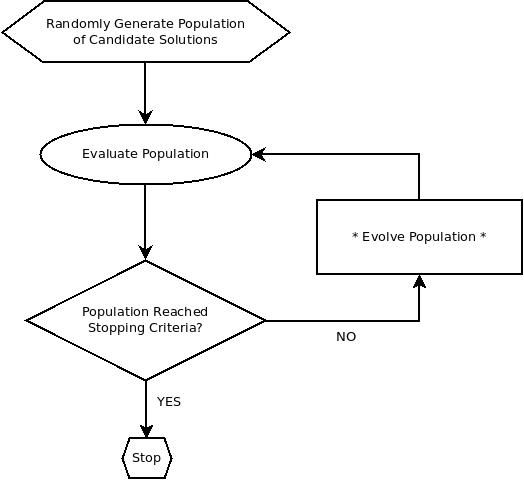
\includegraphics[bb=0 0 524 481,scale=0.5]{figures/EA.jpeg}
	\caption{Population Individual Modification}
	\label{fig:evolutionaryFlowchart}
\end{figure}

\subsection{Population}

The population is a key piece to an EA. Each individual in the population represents a possible candidate solution to the problem that we are attemping to solve. The representation of the individual is usually unique to the problem. Generating the initial population can either be done randomly or by some procedural method. The goal of generating the initial population is to create a diverse\textbf{(CITE)} enough population to find improved solutions.

\subsection{Evaluation Function}
\label{subsec:fitness-function}

This operator determines the fitness of an individual. Each individual is evaluated and given a fitness score to represent how well the individual performed on the problem. This operation is problem specific and it can be very difficult to determine how a problem should be evaluated. The evaluation function is important for differentiating individuals. A poor evaluation function can make each of the individuals appear to be similar when they actually have small key differences. 

\subsection{Stopping Criterion}

Stopping criteria are used to determine when the EA should stop evolving. There are generally three ways stopping criteria can be reached: a maximum number of iterations is reached, the population has converged on the same solution, or the solution has been found.

\subsection{Evolving the Population}

The evolutionary process of an EA is what differs in each implementation of an EA. Each algorithm has a different interpretation of how the population should be evolved. Evolving the population consists of using the individuals in the population to create a new population. Later in this work the different interpretations will be explained.